\begin{frame}{Lower bound method for $\OBDD(\land, \reordering)$}
	Let $\Phi = \bigwedge\limits_{i \in I} C_i$ be minimally unsatisfiable CNF.
    \pause
    \begin{enumerate}
        \item The last step: $\frac{F_1^{\pi} ~~~~ F_2^{\pi}}{0}$. $F_1, F_2$ are satisfiable and
            $F_1 \equiv \bigwedge\limits_{i \in I_1} C_i, F_2 \equiv \bigwedge\limits_{i \in I_2} C_i$
            and $I_1 \neq I_2$, $I_1 \cup I_2 = I$.
        \pause
        \item Find partial substitution $\rho_1, \rho_2$ with same support: $F_1|_{\rho_1} \land
            F_2|_{\rho_2}$ is a hard satisfiable formula for $\OBDD$. Hence either $F_1|_{\rho}^{\pi}$ or
            $F_2|_{\rho}^{\pi}$ is hard for $\OBDD$, hence $F_1$ or $F_2$ is hard for $\OBDD$.
        \pause
        \item $\Phi'$ is a satisfiable formula associated with $\Phi$. Roughly speaking: $\Phi'$ is
            $\Phi$ without several clauses:
            \begin{itemize}
                \item for $\Phi = \PHP^{n + 1}_{n}$, $\Phi' = \PHP^{n}_{n}$;
                \item for unsatisfiable Tseitin formulas, $\Phi'$ is satisfiable Tseitin formula.
            \end{itemize}
        \item Prove that any $\OBDD$ representation of $\Phi'$ has large size.
        
    \end{enumerate}    
\end{frame}


\begin{frame}{Lower bounds for $\OBDD$}
	For particular order $\pi$:
    \begin{itemize}
        \item $F$, $S = \{x_{\pi(1)}, x_{\pi(2)}, \dots, x_{\pi(\ell)} \}$;
        \item let $\rho_1, \rho_2, \dots, \rho_k$ be partial substitution with support $S$ such that
            $F|_{\rho_1}, F|_{\rho_2}, \dots, F|_{\rho_k}$ are different functions;
        \item then every $\pOBDD$ for $F$ has at least $k$ vertices.
    \end{itemize}

    \pause
    For all orders:
    \begin{itemize}
        \item for arbitrary $S$ that consists of $\ell$ variables.
    \end{itemize}

    \pause

    \begin{itemize}
        \item if $(F|_{\rho_i})^{-1}(1), (F|_{\rho_j})^{-1}(1)$ holds forall $i \neq j$ then
            $\CC^{best}_{\ell / n} (F) = \Omega(\log k)$.
    \end{itemize}
    
\end{frame}

\begin{frame}{Pigeonhole principle, $\PHP$}
	\begin{itemize}
        \item $\PHP^m_n$, $m$ pigeons, $n$ holes;
        \item variables $p_{i, j}$, $i \in [m]$, $j \in [n]$, $p_{i, j}$: $i$-th pigeon is in the $j$-th
            hole;
        \item clauses:
        	\begin{itemize}
                \item \color{blue}{long} clauses:
                    $p_{i, 1} \lor p_{i, 2} \dots \lor p_{i, n}$ for all $i \in [m]$;
                \item \color{blue}{short} clauses: $\lnot p_{i, k} \lor \lnot p_{j, k}$ for all $i \neq j
                    \in [m]$ and all $k \in [n]$;
            \end{itemize}
        \item $\PHP^m_n$ is unsatisfiable iff $m > n$.
    \end{itemize}

    \pause
    \begin{lemma}
        \begin{enumerate}
            \item Any OBDD for $PHP^n_n$ has size $2^{\Omega(n)}$.
            \item For all constant $\alpha \le \frac{1}{2}$, $\CC^{best}_{\alpha}(\PHP^n_n) = \Omega(n)$.
        \end{enumerate}
    \end{lemma}

    \pause

    \begin{theorem}
        Any $\OBDD(\land, \reordering)$-proof of $\PHP^{n+1}_n$ has size $2^{\Omega(n)}$.
    \end{theorem}

\end{frame}


\begin{frame}{Tseitin formulas}
	\begin{itemize}
        \item $G(V, E)$ is undirected constant-degree graph;
        \item for every $e \in E$: $x_e$ Boolean variable;
        \item $c: V \to \{0, 1\}$ labelling function;
        \item $TS_{G, c} = \bigwedge\limits_{v \in v} \left( \bigoplus\limits_{u: (u, v) \in E}
            x_{(u, v)} = c(v) \right)$.
    \end{itemize}

    \begin{theorem}[Folklore]
        $TS_{G, c}$ is satisfiable iff for every connected component $U$, $\bigoplus\limits_{v \in U} c(v) = 0$
    \end{theorem}
\end{frame}


\begin{frame}{OBDD for satisfiable Tseitin formula}

    \begin{itemize}
        \item Let $TS_{G, c}$ be satisfiable Tseitin formula;
        \item consider some order $\pi$;
        \item let $S$ be a set that consists first $\ell$ edges according $\pi$;
        \item consider some substitution $\rho$ with support $S$;
        \item $TS_{G, c}|_\rho = TS_{G', c + f}$, where $G'(V, E \setminus S)$ and $f: V \to \{0, 1\}$ is
            a modification of labels made by $\rho$;
        \item different functions: different $f$ and $TS_{G', c + f}$ is satisfiable;
        \item we estimate the number of $f$ such that:
            \begin{itemize}
                \item $TS_{G', c + f}$ is satisfiable;
                \item $f$ can be obtained by a substitution iff $TS_{G'', f}$ is satisfiable, where
                    $G''(V, S)$;
            \end{itemize}
        \item $\sharp G' + \sharp G''$ linear conditions on $f$;
        \item number of different functions at least $2^{n - \sharp G' - \sharp G''}$.
    \end{itemize}
    
\end{frame}


\begin{frame}{Tseitin formulas on expanders}
    \begin{theorem}
        If $G(V, E)$ is good enough expander with $|V| = n$ then $\exists \ell$: $\forall S \subseteq E$
        if $|S| = \ell$ then $\sharp G'(V, E \setminus S) + \sharp G''(V, S) \le (1 - \epsilon) n$.
    \end{theorem}

    \pause

    \begin{corollary}
        Every $\OBDD$ representation of satisfiable $TS_{G, c}$ has size at least $2^{\Omega(n)}$.
    \end{corollary}

    \pause

    \begin{corollary}
        If $G$ differs from good enough expander by at most $o(n)$ edges, then $\OBDD$ representation of
        satisfiable $TS_{G, c}$ has size at least $2^{\Omega(n)}$.
    \end{corollary}

    \begin{lemma}
        Good enough expander is connected and remains connected after deleting of any two vertices and
        edges from the shortest path between them.
    \end{lemma}
\end{frame}

\begin{frame}{Lower bound for unsatisfiable Tseitin formula}
    \begin{theorem}
    	If $G(V, E)$ is good enough expander with $|V| = n$ and $TS_{G, c}$ is unsatisfiable then the
        size of any $\OBDD(\land, \reordering)$-proof of $TS_{G,c}$ is at least $2^\Omega(n)$.
    \end{theorem}

	\begin{columns}[t]
		\begin{column}{0.45\textwidth}
            \begin{itemize}
                \item The last step: $\frac{F_1^{\pi} \land F_2^{\pi}}{0}$. $F_1, F_2$ are satisfiable.
                \item Let $F_1$ does not contains $C_u$ and $F_2$ does not contain $C_v$ and $(u, v)
                    \notin E$.
                \item $P$ is the shortest $uv$-path.
            \end{itemize}    
        \end{column}
        
		\begin{column}{0.45\textwidth}
            \begin{figure}[ht]
                \begin{center}
                    \scalebox{0.35}{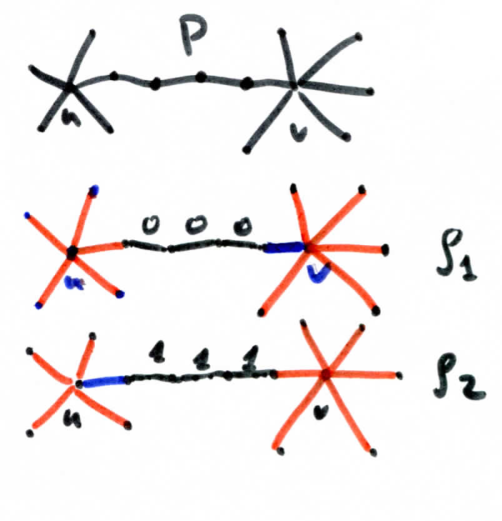
\includegraphics{pics/tseitin.pdf}}
                \end{center}
                $F_1|_{\rho_1} \land F_2|_{\rho_2}$ is almost satisfiable $TS_{\tilde G, c'}$, where
                $\tilde G(V\setminus\{u,v\},E\setminus P)$.
            \end{figure}
		\end{column}
	\end{columns}
\end{frame}

\begin{frame}
	\begin{enumerate}
        \item Lower bound for $\OBDD(\land, \weakening, \reordering)$-proofs.
        \item Does $\OBDD(\land, \weakening)$ simulate $\OBDD(\land, \reordering)$?
        \item Is it possible to simulate $\OBDD(\land)$-proofs by $\OBDD(\land, \exists)$-algorithms?
        \item Prove lower bound for $\OBDD(\land, \exists, \reordering)$-algorithms on unsatisfiable
            linear systems.
    \end{enumerate}    
\end{frame}
